\documentclass{article}
\usepackage{polski}
\usepackage[utf8]{inputenc}
\usepackage{graphicx} % Required for inserting images
\usepackage[polish]{babel}
\usepackage{amsmath}
\usepackage{amsfonts}
\usepackage{amssymb}
\usepackage{polski}
\usepackage{indentfirst}
\usepackage{graphicx}
\usepackage{placeins}
\usepackage{makecell}
\usepackage{float}
\usepackage{hyperref}



% wymiary strony
\setlength{\textheight}{24cm}
\setlength{\textwidth}{16.92cm}
\setlength{\footskip}{10mm}
\setlength{\oddsidemargin}{-0.5cm}
\setlength{\evensidemargin}{-0.5cm}
\setlength{\topmargin}{0mm}
\setlength{\headsep}{5mm}
\setlength{\parskip}{5mm}

\title{Optyczne - Grodzki}
\author{Piotr Janiszewski}
\date{January 2025}

\begin{document}

\maketitle
\tableofcontents
\newpage

\section{Wykład 1 - Wprowadzenie}
\subsection{Porównanie metod dostępu do sieci Internet.}
W czasach łączy miedzianych najczęściej używaną techniką dostępową było \textbf{xDSL} (ADSL i VDSL) bazujące na architekturze punkt-punkt.\\
\textbf{VDSL} (szybszka wersja ADSL)
\begin{itemize}
  \item Teoretyzne \textbf{52 Mb/s} każdemu użytkownikowi
  \item Maksymalna odległość do abonenta przy makssymalnej przepustowości to \textbf{300m}
\end{itemize}

\textbf{ADSL2} (zwiększenie zasięgu) \\
\textbf{VDSL2}
\begin{itemize}
    \item Do 300m prędkość: 200 Mb/s
    \item Po 500m prędkość: 100 Mb/s
    \item Po 1km prędkość: 50 Mb/s
\end{itemize}

\subsection{Dlaczego światłowód?}
Pomimo popularności to rozwój telewizji wymagały szybszego łącza (StandardTV to 2 Mb/s a HDTVSuper (4k) to już 50 Mb/s.\\
Szacunkowe analizy wymaganego przez pakiet z telewizją wysokiej rozdzielczości wymagają 30-50 Mb/s, a w przyszłości 100 Mb/s dla każdego abonenta.
Wymagania te przewyższają możliwości medium miedzianych.\\
Rozwiązaniem problemu jest budowa sieci w technice FTTx. Sieć charakteryzuje się połączeniem światłowodem pomiędzy obiektami centralowymi i do punktów dystrybyucyjnych z których idzie sieć miedziana do użytkowników.\\
Sieć FTTx dzięki używaniu w większości urządzeń pasywnych jest tańsza w ekspoatacji od sieci opartych o kable miedziane.

\subsection{Większe pasmo, nowe pomysły na usługi. }
\begin{enumerate}
  \item Internet
  \item Telewizja i VOD
  \item Gry-Online
  \item Usługi chmurowe
  \item Moinitoring
  \item Wirtualne biuro / e-learning
  \item Opieka medyczna\ldots
\end{enumerate}
\section{Wykład 2 - Sieć telekomunikacyjna, podział sieci.}
\textbf{Sieć telekomunikacyjna} to ogól węzłów, linie telekomunikacyjne, łącza między węzłami, których celem jest nadawanie, odbiór lub transmisja danych.
\begin{figure}[h!]
    \centering
    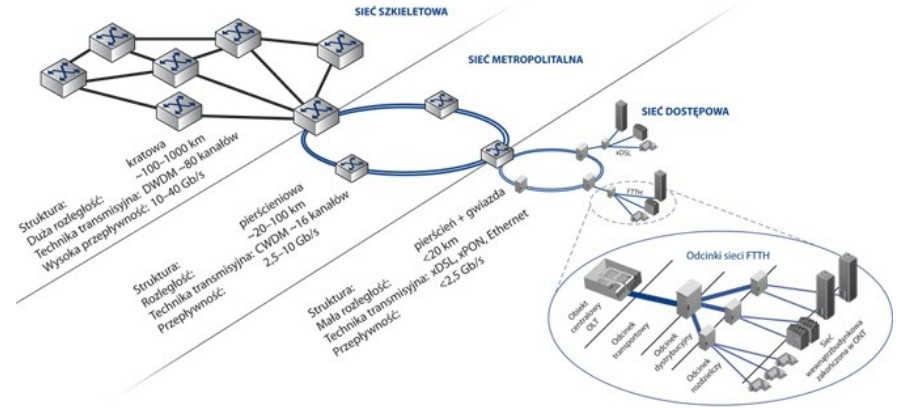
\includegraphics[width=0.7\linewidth]{w02z01.jpg}
    \caption{Segmenty sieci FTTH}
    \end{figure}
\textbf{Podsział sieci ze wzglęcu na zasięg:}
\begin{enumerate}
    \item \textbf{WAN} - sieć szkieletowa (Wide Area Network)
    \item \textbf{MAN} - sieć metropolitalna (Metropolian Area Network)
    \item \textbf{CAN} - sieć akademicka (Campus Area Network)
    \item \textbf{LAN} - sieć lokalna (Local Area Network)
\end{enumerate}
\subsection{Sieci optyczne pierwszej generacji}
\textbf{Lata 70-e:}
\begin{enumerate}
    \item[$\blacksquare$] Wytworzenie pierwszego światłowodu o małych stratach.
    \item[$\blacksquare$] Początek sieci optycznych typu punkt-punkt.
    \item[$\blacksquare$] Regeneracja sygnały odbywa się elektronicznie.
    \item[$\blacksquare$] Wykorzystywanie do przesyłania rozmów telefonicznych.
    \item[$\blacksquare$] Technologia wykorzystywana w sieciach PDH.
\end{enumerate}
\textbf{PDH (Plesiochronus Digital Hierarchy):} Sieć prawie zsynchronizowana, każdy węzeł ma swój zegar, które nie są z sobą doskonale zsynchronizowane.
\begin{figure}
    \centering
    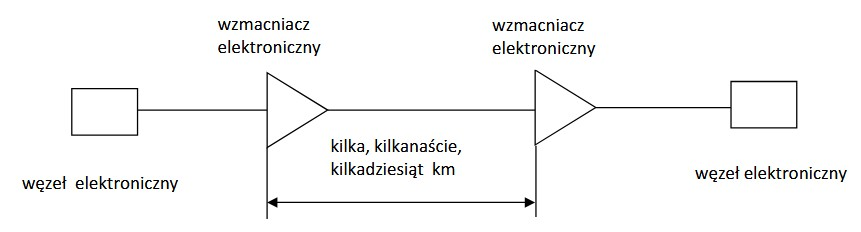
\includegraphics[width=0.7\linewidth]{w02z02.jpg}
    \caption{Sieć PDH}
\end{figure}
\newpage
\textbf{Lata 80-e}
\begin{enumerate}
    \item[$\blacksquare$] Sieć SONET / SDH (Synchronous Optical NETwork - Synchroniczna sieć optyczna / Synchronous Digital Hierarchy - Synchroniczna Hierarchia Cyfrowa.
    \item[$\blacksquare$] Początki prac nad wzmacniaczami optycznymi.
    \item[$\blacksquare$] Początki prac nad multipleksacją falową (WDM).
\end{enumerate}

\subsection{Sieci optyczne drugiej generacji}
\textbf{Lata 90-e:}
\begin{enumerate}
    \item[$\blacksquare$] Opracowanie sieci optycznych drugiej generacji
    \item[$\blacksquare$] Najważniejsza cecha \textbf{Komutacja optyczna.}
    \item[$\blacksquare$] Cechy dodatkowe:
        \begin{itemize}
            \item Zastosowanie wzmaczniaczy optycznych.
            \item Zastosowanie multipleksacji falowej (WDM).
        \end{itemize}
\end{enumerate}
\begin{figure}[H]
    \centering
    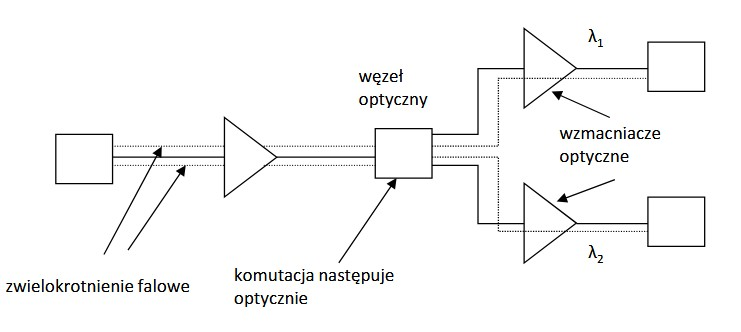
\includegraphics[width=0.7\linewidth]{w02z03.jpg}
    \caption{Sieć drugiej generacji}
\end{figure}

\newpage
\subsection{Sieci optyczne jako połączenie optyki i elektroniki: Zalety i wady} 
\begin{table}[H]
    \caption{Wady i zalety sieci optycznych i elektronicznych}
    \centering
    \begin{tabular}{ccc}
    \hline
         & Zalety & Wady \\
         \hline
        Optyka  & Odporność na interferencje & Słabe możliwości obliczeniowe\\
                & Mała tłumienność &  Brak możliwości przechowywania światła \\
        \hline
        Elektronika & Bardzo dobre możliwości obliczeniowe & Brak odporności na interferencje\\
                    & Możliwość ,,przechowywania" w pamięci RAM & Duża oporność kabla (słaby zasięg)\\
    \end{tabular}    
    \label{tab:my_label}
\end{table}
\underline{\textbf{Wnioski:}} \\
Optyka - Transmisja na duże odległości\\
Elektronika - Przetwarzanie danych

\section{Wykład 3 - Media światłowodowe.}
\subsection{Światłowód - definicja}
Falowód służy do przesyłania promieniowania świetlnego. Zasada działania opiera się na transmisji impulsów świetlnych między nadajnikiem przekazującym sygnały elektryuczne na świetle, a odbiornikiem przekształcający sygnały świetlne odebrane w sygnały elektryczne. Sieci oparte na światłowodach zwane są \textbf{FDDI (Fiber Distributed Data Interface).}
\subsection{Budowa kabli światłowodów}
\begin{figure}[H]
    \centering
    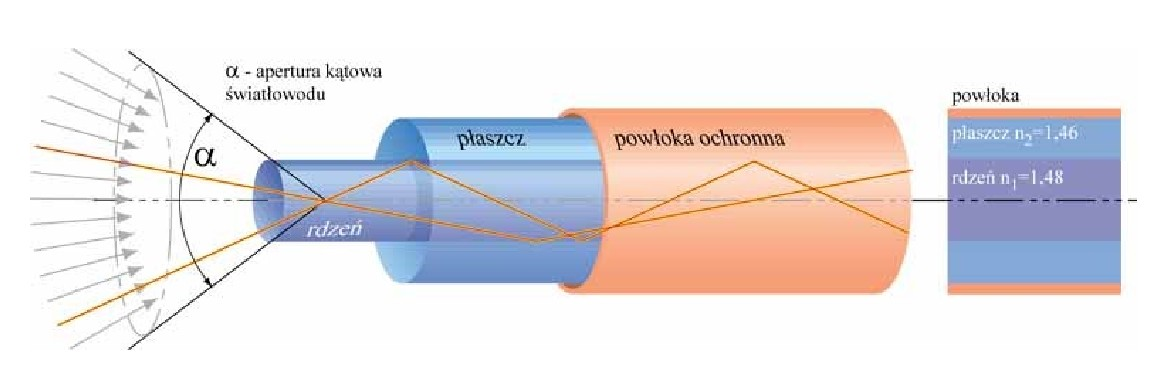
\includegraphics[width=0.7\linewidth]{w03z01.jpg}
    \caption{Budowa kabla}
\end{figure}
\textbf{Rdzeń} (Core) znajduje się pośrodku kabla. Wykonany jest ze szkła kwarcowego lub plastiku. Średnica: 9 minronów dla jednomodowych i do 50 lub 62.5 mikronów dla wielomodowych światłowodów.

\textbf{Płaszcz} (Cladding) wykonany z materiału o niższym współczynniku załamania światła od rdzenia. Zachowuje się niczym lustro kierując promień do wnętrza formując falę.

\textbf{Powłoka lakierowa / bufor} (Buffer Coating) chroni warstwę płaszcza. Wykonany z materiałów termoplastycznych. Chroni przed uszkodzeniami mechanicznymi. Kabel pod wpływem temperatury może sie wydłużać lub skracać.
\subsection{Działanie światłowodu}
\begin{itemize}
    \item Promień światła wędrując w rdzeniu o współczynniku załamania n\textsubscript1, napotyka na środowisko o innym współczynniku załamania n\textsubscript2 - płaszcz.
    \item Gdy promień pada od strony rdzenia na płaszcz pod kątem alfa, to część światła zostaje odbita i wraca do rdzenia.
    \item W zależności od kąta i współczynników załamania materiałów zmienia się ilość odbitego światła. Powyżej pewnego kąta zachodzi zjawisko całkowitego odbicia wewnętrznego i światło zostaje odbije bez strat.
\end{itemize}

\subsection{Rodzaje światłowodów}
\subsubsection{Światłowody jednomodowe}
Światłowody jednomodowe (Single Mode Fiber - SMF).

W światłowodach jednomodowych sygnał ulega niewielkim zniekształceniom w wyniku \textbf{dyspersji chromatycznej}, na którą składają się 2 zjawiska: dyspersja \textbf{materiałowa i falowa:}
\begin{itemize}
    \item \textbf{Dyspersja materiałowa} - spowodowana jest zmianą współczynnika załamania szkła kwarcowego w funkcji długości fali.
    \item \textbf{Dyspersja falowa} - częściowo spowodowana jest wędrowaniem wiązki przez płaszcz światłowodu.
\end{itemize}

\begin{figure}[H]
    \centering
    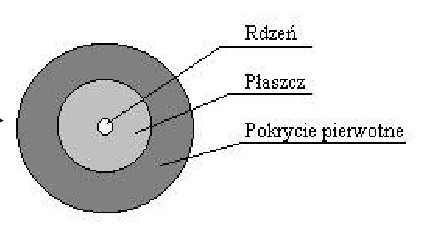
\includegraphics[width=0.4\linewidth]{w03z02.jpg}
    \caption{Przekrój włókna światłowodu jednomodowego}
\end{figure}

\begin{itemize}
    \item Fala rozchodzi się równolegle do osi światłowodu.
    \item Mała średnica rdzenia 9 mikronów
    \item Skokowa zmiana współczynnika światła.
    \item Źródło światła - laser.
    \item Do dalekosiężnej telekomunikacji (do 100km bez wzmacniania).
    \item Żywotność - 25 lat
    \item Droga
\end{itemize}
\paragraph{Wydajność wzrasta ze wzrostem długości fali, ale wzrastają koszta.}

\subsubsection{Światłowody wielomodowe}
Światłowody wielomodowe (Multi Mode Fiber - MMF).\\
Charakteryzują się średnicą 50 lub 62,5 mikrometra. W światłowodzie wielomodowym następuje rozdzielenie fali wejściowej na wiele promieni o takiej samej długości lecz propagowanymi po innych drogach.\\
Występuje zjawisko zniekształcenia impulsu wyjściowego co powoduje ograniczenie prędkości i odległości transmisji.\\
\begin{figure}[H]
    \centering
    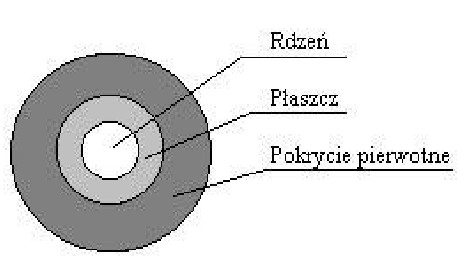
\includegraphics[width=0.4\linewidth]{w03z03.jpg}
    \caption{Przekrój włókna światłowodu wielomodowego}
\end{figure}
\textbf{Światłowody dzielimy na skokowe i gradientowe}

\paragraph{Światłowód gradientowy} ma budowę warstwową. Każda jest inaczej domieszkowana, dzięki czemu współczynnik załamania zmienia się w sposób ciągły.\\
Zapewniają te samą prędkość dla różnych modów. Dzieje się tak bo mniejszy współczynnik załamania oznacza większą prędkość liniową.
\begin{figure}[H]
    \centering
    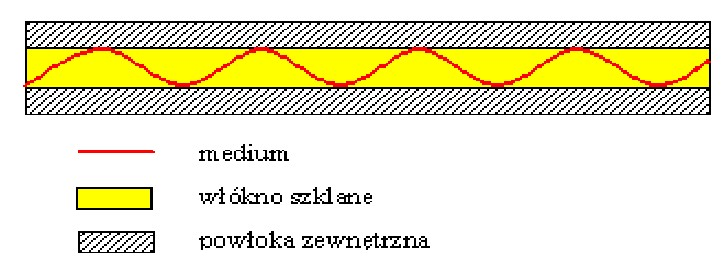
\includegraphics[width=0.6\linewidth]{w03z04.jpg}
    \caption{Przekrój światłowodu gradientowego}
\end{figure}
\newpage
\paragraph{Światłowód skokowy:} Współczynnik załamania zmienia się skokowo pomiędzy rdzeniem i płaszczem. Mody są prowadzone pod różnymi kątami, przez co mają różną drogę do przebycia. Prędkość światła jest stała dlatego czasy są różne.
\begin{figure}[H]
    \centering
    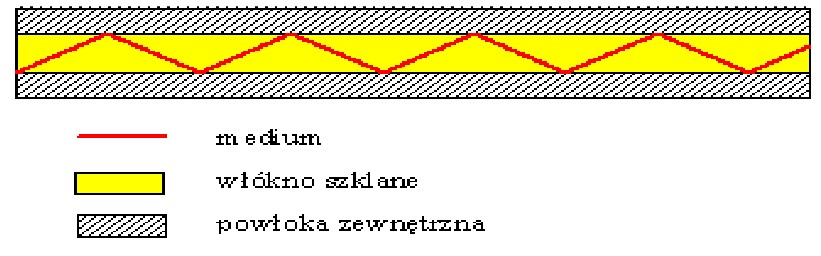
\includegraphics[width=0.6\linewidth]{w03z05.jpg}
    \caption{Przekrój światłowodu skokowego}
\end{figure}
\hrule
\begin{figure}[H]
    \centering
    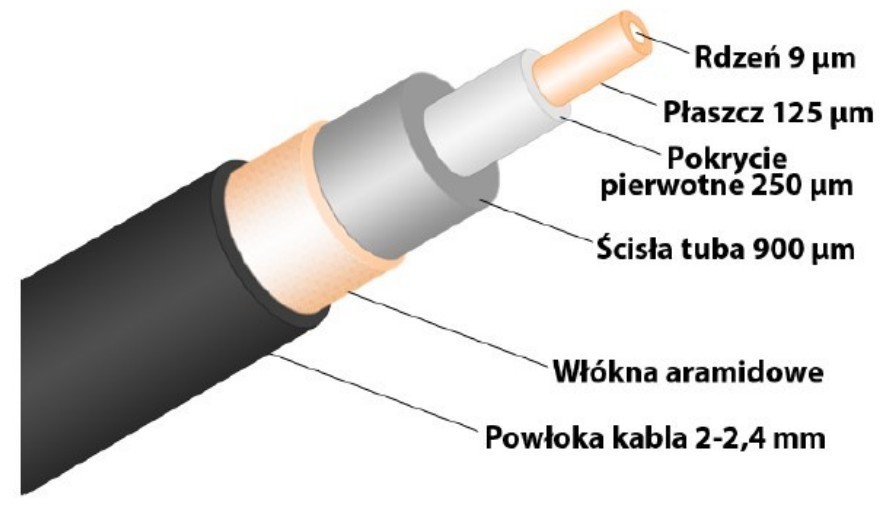
\includegraphics[width=0.6\linewidth]{w03z06.jpg}
    \caption{Budowa kabla światłowodowego}
\end{figure}
\subsection{Rodzaje ze względu na konstrukcje:}
\begin{enumerate}
    \item Zipcord: Prosta płaska konstrukcja składający się zazwyczaj z dwóch włókien umieszczonych równolegle i połączonych cienką warstwą osłony. Głównie do krótkich połączeń wewnątrzbudynkowych.
    \item Distribution (kabel dystrybucyjny): Wiele włókien w jednej osłonie, bez buforów dla każdego włókna.\\ Stosowany w instalacjach wewnątrzbudynkowych (np. w pionach i szafach telekomunikacyjnych)
    \item Loose Tube (Luźna tuba): Włókna w żelu ochronnym chroniącym przed wilgocią i naprężeniem mechanicznym. Tuba zawiera jedno lub kilka włókien.\\ \textbf{Stosowana głównie na zewnątrz} (kanalizacja, pod ziemią)
    \item Breakout (kabel rozgałęźny): Każde włókno posiada własny bufor ochronny a całość w dodatkowej osłonie. Bardziej odporny na uszkodzenia mechaniczne i używany w trudniejszych warunkach jak zakłady przemysłowe czy serwerownie. \textbf{Mniej elastyczny niż distribution}
\end{enumerate}

\section{Wykład 5 - Napowietrzne sieci światłowodowe.}
\subsection{Technologie traktów światłowodowych:}
\textbf{OPGW} (Optical Ground Wire)\\
Przewody odgromowe linii energetycznych ze światłowodami wewnątrz konstrukcji w tubach metalowych. Stosowane w liniach 110 kV wzwyż.

\textbf{OPCON, OPPC} (Optical Phase Conductor), \textbf{MASS} (Metalic Aeral Self Supporting Cable)\\
Przewody fazowe ze zintegrowanymi tubami światłowodowymi stosowane na liniach niskiego, średniego i wysokiego napięcia. Konstrukcje te same co w przypadku OPGW
\begin{figure}[H]
    \centering
    
\includegraphics[width=0.6\linewidth]{w05z01.jpg}
    \caption{Przykład OPCON}
\end{figure}

\textbf{ADSS} (All Dielectric Self Supporting Cable)\\
Samonośne kable światłowodowe podwieszane, stosowane na liniach do 110 kV. Wykonywane są jako całkowicie dielektryczne.
\begin{figure}[H]
    \centering
    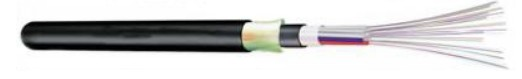
\includegraphics[width=0.6\linewidth]{w05z02.jpg}
    \caption{Przykład ADSS}
\end{figure}

\textbf{ADL} (All Dielectric Lashed), \textbf{SkyWrap}\\
Kable światłowodowe owijane wokół przewodów fazowych lub odgromowych i mocowane do nich przy pomocy oplotu taśm.
\begin{figure}[H]
    \centering
    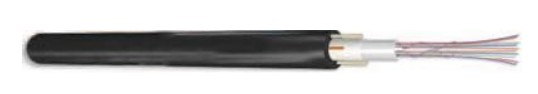
\includegraphics[width=0.6\linewidth]{w05z03.jpg}
    \caption{Przykład ADL}
\end{figure}
\newpage
\subsection{OPGW - Optical Ground Wire}
Przewody odromowe linii energetycznych ze światłowodami umieszczonymi wewnątrz konstrukcji w tubach metalowych.
\textbf{Zastosowanie:} linie od 100 kV wzwyż.\\
\textbf{Podstawowa konstrukcja:} aluminiowa, nie korodująca, centralna tuba, wewnątrz której biegną włókna światłowodowe lub pęczki włókien.
\begin{itemize}
    \item Spotykane z dodatkową tubą plastikową wewnątrz tuby aluminowej. Zapewnia to dużą wytrzymałość
    \item Stosuje się także konstrukcje z dwoma lub trzeba tubami zawierającymi światłowody umieszczone pomiędzy rurami.
    \item Przewód OPGW jest odporny na zjawisko "płynięcia".
\end{itemize}
\begin{figure}[H]
    \centering
    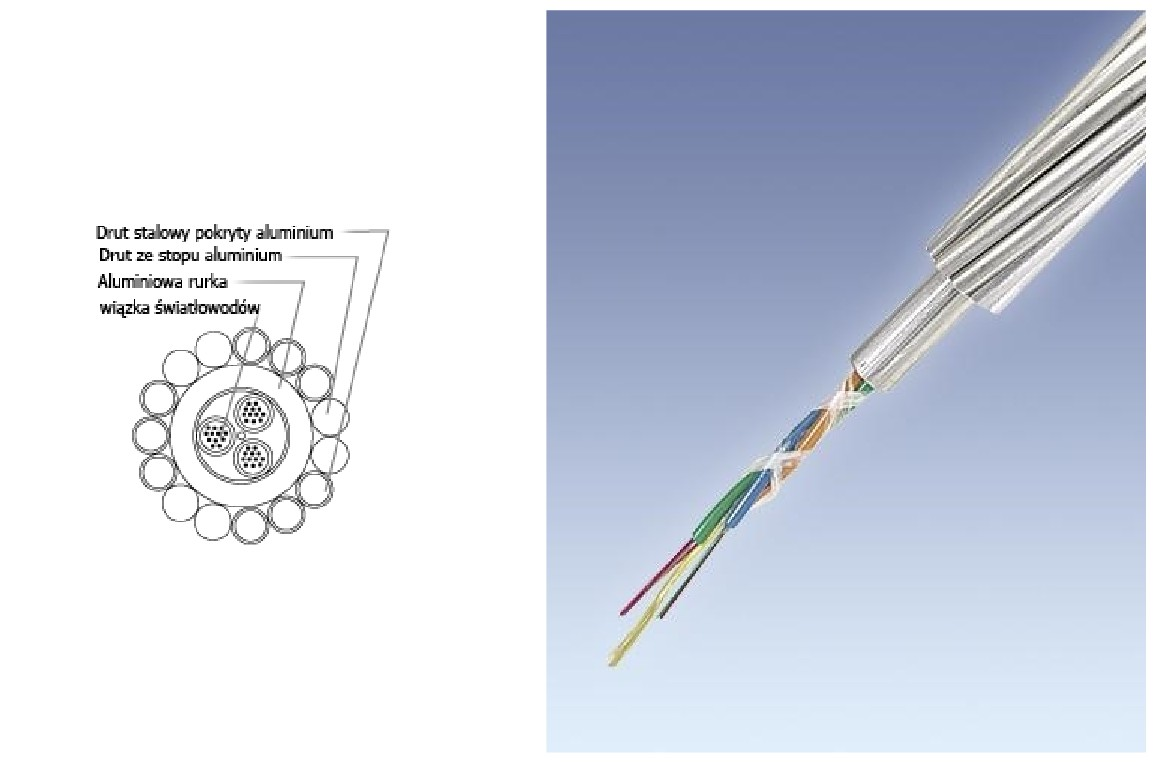
\includegraphics[width=0.6\linewidth]{w05z04.jpg}
    \caption{Konstrukcja kabla OPGW}
\end{figure}
\begin{figure}[H]
    \centering
    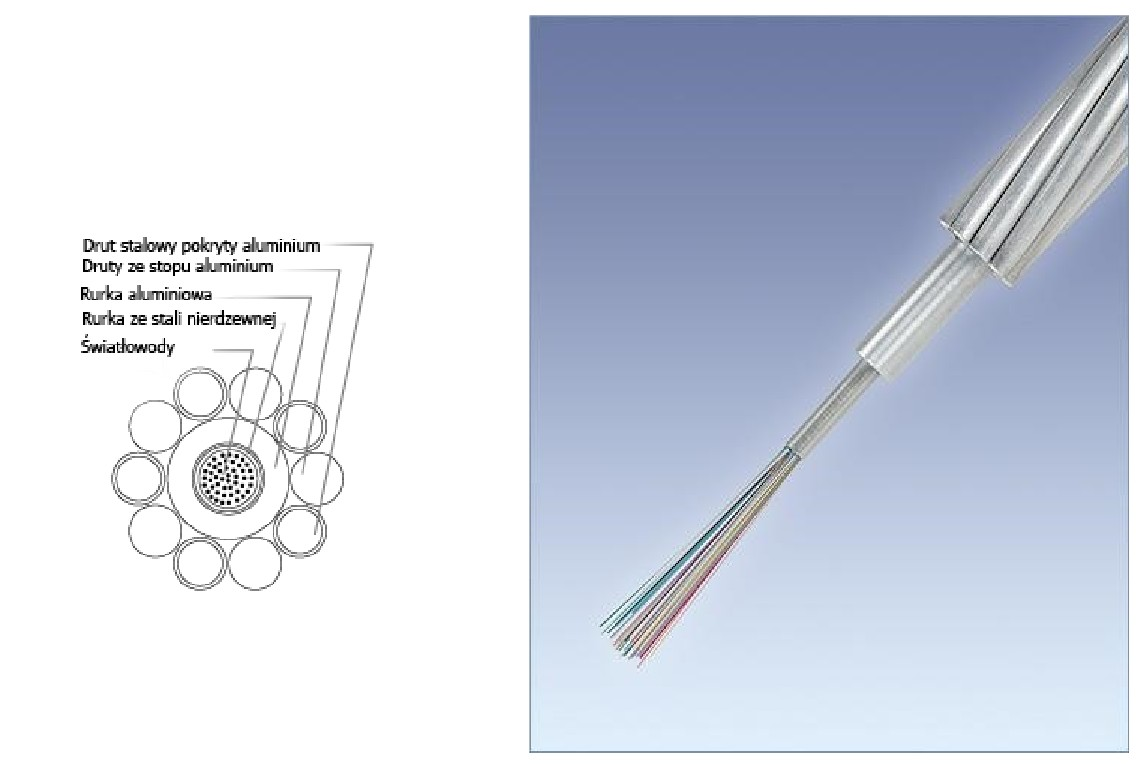
\includegraphics[width=0.6\linewidth]{w05z05.jpg}
    \caption{Konstrukcja kabla OPGW}
\end{figure}
\begin{figure}[H]
    \centering
    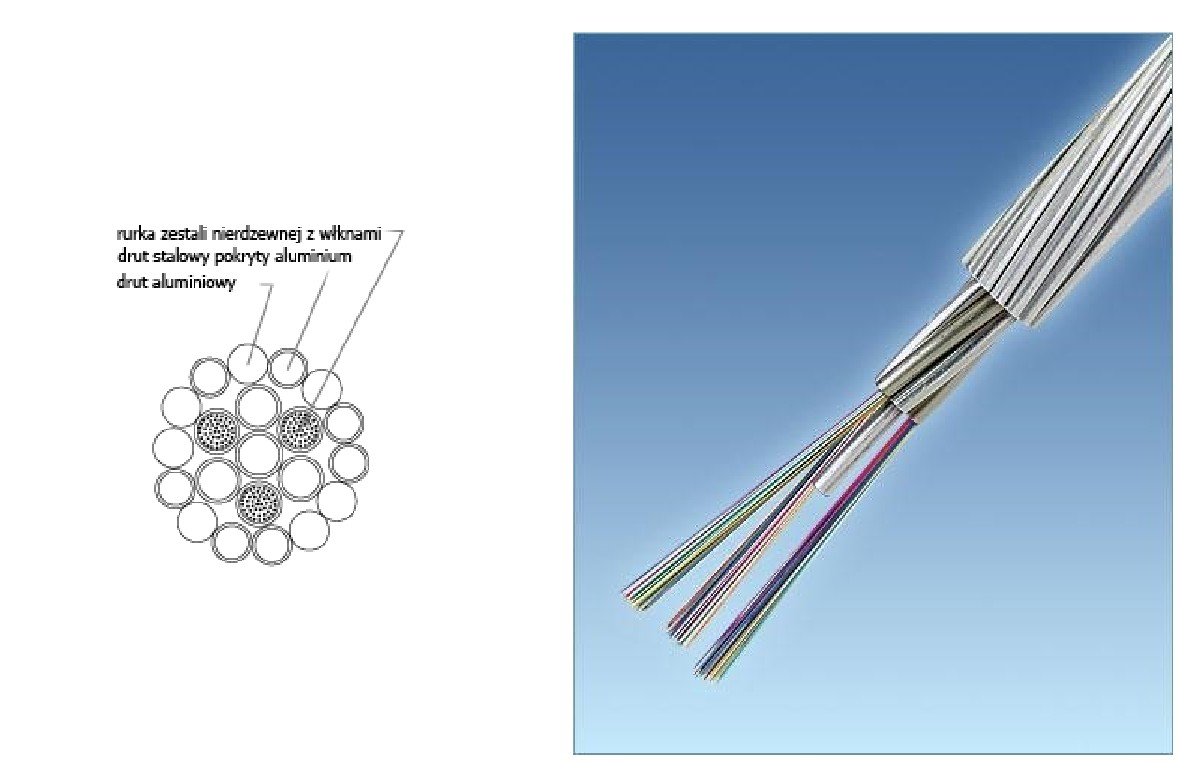
\includegraphics[width=0.6\linewidth]{w05z06.jpg}
    \caption{Konstrukcja kabla OPGW}
\end{figure}
\begin{figure}[H]
    \centering
    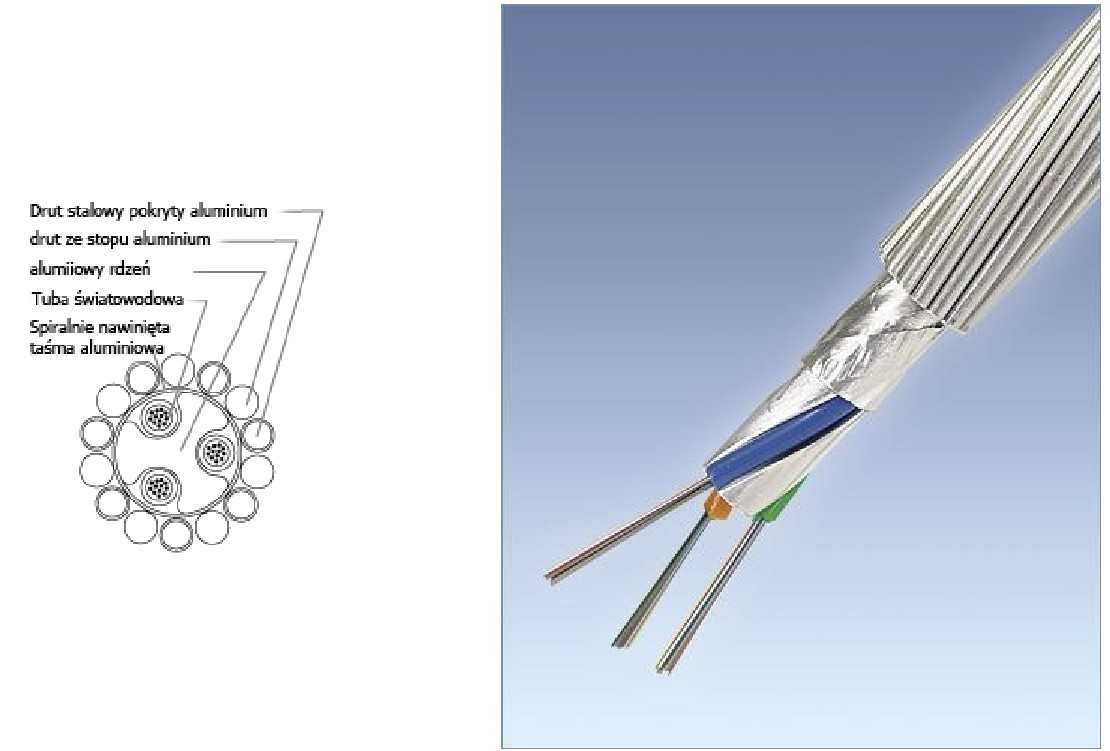
\includegraphics[width=0.6\linewidth]{w05z07.jpg}
    \caption{Konstrukcja kabla OPGW}
\end{figure}
\newpage
\subsection{OPCON, OPPC - Optical Phase Conductor, MASS – Metalic Areal Self Supporting Cable}
Przewody fazowe ze zintegrowanymi tubami światłowodowymi stosowane na liniach niskiego i średniego
napięcia.

\textbf{Konstrukcja:} ta sama co w przypadku przewodów OPGW.
Stosuje się inny osprzęt (do pracy pod napięciem), uwzględnia się parametry elektryczne przewodów nominalnych i zwarciowych.\\
Kosztowniejsza budowa linii przez użycie osprzętu izolujący część telekomunikacyjną od wysokich napięć.\\
Napięcie odstrasza złodziei.

\textbf{Zalety}
\begin{itemize}
    \item Wysoka odporność na czynniki mechaniczne i elektryczne.
    \item Możliwość zastosowania dużej ilości włókien
    \item Mała średnica zewnętrzna
    \item Większa długość nadmiarowa włókien w aluminiowej tubie
    \item Duża odporność na warunki temperaturowe
    \item Linię telekomunikacyjną montuje się wymieniając istniejące przewody
    \item Niski koszt realizacji w przypadku instalacji na nowych liniach
\end{itemize}

\textbf{Wady}
\begin{itemize}
    \item Możliwość awarii rozległych przez huragany, oblodzenie,
    \item Długie czasy napraw związane z koniecznościa wyłączenia linii energetycznych.
    \item Złącza można instalować jedynie na słupach mocnych.
    \item Umieszczone na słupach złącza są narażone na wandali.
\end{itemize}

\subsection{ADSS - All Dielectric Self Supporting Cable}
Montowane na osi słupów poniżej przewodów roboczych. Mogą być w kanalizacji kablowej i w ziemi co upraszcza budowę linii.

\textbf{Zalety}
\begin{itemize}
    \item Szybka i tania instalacja
    \item Wykorzystuje istniejącą infrastrukture linii energetycznych
    \item Tani osprzęt.
    \item Typowe narzędzia do wykonywania złączy
    \item Możliwa naprawa bez wyłączania linii
\end{itemize}

\textbf{Wady}
\begin{itemize}
    \item ADSS powoduje zmiany obciążenia słupów co wymaga ponownego obliczenia wytrzymałości linii i często wzmocnienie słupów
\end{itemize}

\subsection{ADL - All Dielectric Lashed, SkyWrap}
Kable światłowodowe mocowane do przewodów fazowych lub odgromowych przy pomocy oplotu z taśm lub sznurów. Lekkie, o niewielkich średnicach, często z centralną tubą, projektowane w sposób nie powodujący znacznych zmian w obciążeniu słupów.

\textbf{SkyWrap - produkcja AFL}
To kabel światłowodowy spiralnie montowany na przewodach odgromowych lub fazowych linii energeycznych. Specjalnie skonstruowana maszyna jest używana do owijania kabla przy zachwoaniu ścisłej kontroli parametrów. SkyWrap jest indelanym rozwiązaniem kiedy dostęp do linii jest utrudniony. Urządzeniqa są lekkie i łatwe w obsłudze. Nie wymaga wyłączenia linii.

\textbf{Zalety}
\begin{itemize}
    \item Szybka i tania instalacja.
    \item Wykorzystanie istniejącej infrastruktury.
    \item Możliwa instalacja w miejscach utrudnionych.
    \item Można instalować na przewodach odgromowych i fazowych.
\end{itemize}

\textbf{Wady}
\begin{itemize}
    \item Niska żywotność (7-15 lat).
    \item Przerwane oploty ADL powodują zwarcia.
    \item Kable na przewodach odgromowych ulegają uszkodzeniu podczas uderzenia pioruna.
    \item Kable zainstalowane na przewodach fazowych ulegają przepaleniu podczas zwarcia spowodowanego dotnięciem gałęci.
\end{itemize}

\begin{figure}[H]
    \centering
    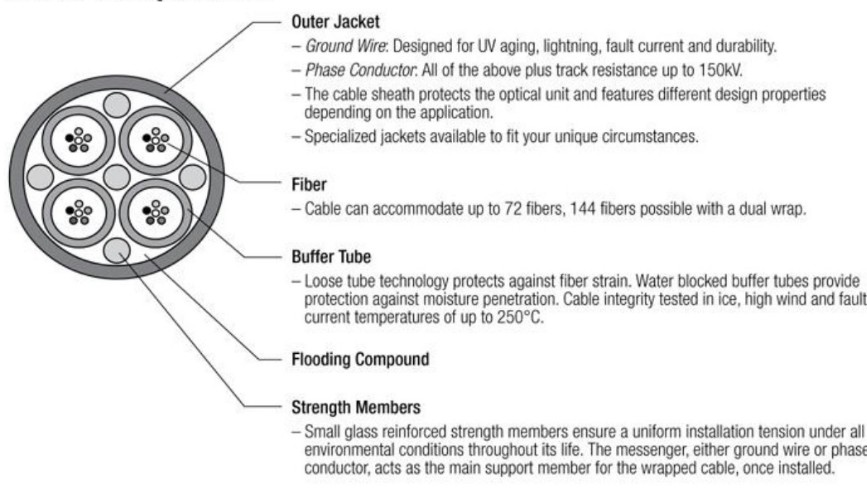
\includegraphics[width=0.6\linewidth]{w05z08.jpg}
    \caption{Konstrukcja kabla ADL}
\end{figure}

\section{Wykład 6 - Instalacje sieci FTTH.}
\subsection{Przegląd technologii FTTx ( FTTCab, FTTC, FTTB, FTTH).}
\subsection{Elementy infrastruktury FFTH}
\subsection{Podział funkcjonalny kabli światłowodowych}
\subsection{Mikrokable w sieciach FTTH.}
\subsection{Kanalizacja teletechniczna}
\subsection{Mikrokanalizacja.}
\subsection{Studnie kablowe i zasobniki kablowe.}
\subsection{Osłony złączowe, mufy.}
\subsection{Szafy dystrybucyjne uliczne z wyposażeniem, skrzynki hermetyczne.}














\section{Wykład 7 - Infrastruktura wewnątrzbudynkowa.}
\subsection{Skrzynki i przełącznice wewnątrz budynkowe dystrybucyjne i zakończeniowe.}
\subsection{Okablowanie budynków wielokondygnacyjnych.}
\subsection{Gniazda abonenckie i światłowodowe patchcordy przyłączeniowe.}
\subsection{Multimedialne domowe skrzynki rozdzielcze.}
\subsection{Infrastruktura punktu styku sieci FTTH z siecią metropolitarną.}
\newpage
\section{Wykład 8 - Architektura FTTH}
\subsection{Sieci P2P i P2MP}
\subsection{Urzadzenia centralowe - OLT}
\subsection{Terminal abonencki - ONT}
\subsection{Ewolucja sieci P2MP (BPON, EPON, GPON.)}
\subsection{Porównanie sieci P2P i P2MP.}
\subsection{Wybrane aspekty projektowania, budowy i eksploatacji sieci FTTH.}
\subsection{Zarządzenie włókniami i okablowaniem}

\section{Wykład 9 - Wymiarowanie optyczne łącza - budżet mocy optycznej.}
\subsection{Bilans mocy optycznej.}
\subsection{Planowanie układów splitterów w sieci.}
\subsection{Zapewnienie dostępu abonenta do usług innego operatora.}
\subsection{Instalacje wewnątrzbudynkowe - techniki okablowania budynku (technika klasyczna, kabla łatwego dostępu, w wykorzystaniem mikrokanalizacji ).}
\subsection{Zakończenie abonenckie.}
\subsection{Szablony rozwiązań dla budynku wielorodzinnego.}
\subsection{Szablony rozwiązań dla budynku jednorodzinnego.}
\newpage
\section{Wykład 10 - Pomiary toru optycznego w sieciach FTTH.}
\subsection{Elementy toru optycznego - włókno światłowodowe.}
\subsection{Pomiary reflektometrem.}
\subsection{Elementy toru optycznego - połączenia trwałe (spawy termiczne, łączniki mechaniczne).}
\subsection{Elementy toru optycznego - połączenia rozłączne (złącza światłowodowe).}
\subsection{Wymagania odnośnie pomiarów i pracy z systemami światłowodowymi.}
\subsection{Pomiary w sieciach FTTH (na etapie budowy sieci i instalacji osprzętu, na etapie utrzymania sieci, serwisowe).}
\subsection{Pomiary mocy i transmisji.}
\subsection{Analiza wyników pomiarów reflektometrycznych.}

\section{Wykład 11}
\subsection{Multipleksowanie z podziałem czasu TDM.}
\subsection{Multipleksowanie z podziałem częstotliwości FDM.}
\subsection{Multipleksowanie kodowe CDM.}
\subsection{Multipleksowanie z podziałem długości fali WDM.}
\subsection{Rodzaje zwielokrotniania WDM (CWDM, DWDM, UWDM).}
\subsection{Wykorzystanie wzmacniacza EDFA.}
\subsection{Komponenty optyczne}
\subsection{Podstawowe struktury sieci optycznych (pasywna gwiazda, pasywny router, aktywny przełącznik, aktywny przełącznik z konwersją długości fali).}


\end{document}
